% ===== 4 筛分语义映射 =====
\section{从二维视觉到标准筛分级配}
\label{sec:r-sieve}

\subsection{二维视觉粒径不等于筛孔粒径}

机械筛分判断的是三维颗粒在振动和姿态变化过程中能否通过给定筛孔，而单目相机只能观测当前姿态下的二维投影。因此，某个二维长度可以作为筛分行为的代理，但不能未经验证地与筛孔尺寸画等号。图\ref{fig:r-sieve-semantics}示意了两者的物理差异：相机得到的是当前视角的投影椭圆和可见轮廓；机械筛分则允许颗粒在三维中旋转并寻找可通过筛孔的姿态，决定通过行为的尺度可能同时受短轴、厚度、形状和姿态影响。

\begin{figure}[t]
\centering
\begin{tikzpicture}[
  box/.style={rectangle,draw,rounded corners,minimum width=4.0cm,minimum height=2.1cm,align=center,font=\footnotesize},
  arr/.style={->,thick}
]
\node[box,fill=gray!7] (grain) {\begin{tikzpicture}[scale=0.7]
\draw[thick,rotate=15] (0,0) ellipse (1.25 and 0.72);
\draw[dashed,rotate=15] (0,0) ellipse (1.25 and 0.32);
\draw[<->] (-1.15,-0.95)--(1.15,-0.95) node[midway,below,font=\scriptsize] {三维尺寸与姿态};
\end{tikzpicture}\\真实颗粒};
\node[box,fill=blue!7,right=0.8cm of grain] (proj) {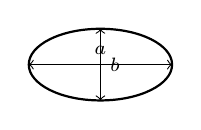
\begin{tikzpicture}[scale=0.7]
\draw[thick] (0,0) ellipse (1.3 and 0.65);
\draw[<->] (-1.3,0)--(1.3,0) node[midway,above,font=\scriptsize] {$a$};
\draw[<->] (0,-0.65)--(0,0.65) node[midway,right,font=\scriptsize] {$b$};
\end{tikzpicture}\\单目二维投影};
\node[box,fill=orange!8,right=0.8cm of proj] (sieve) {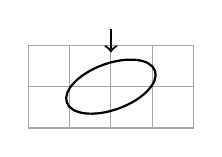
\begin{tikzpicture}[scale=0.7]
\draw[step=0.75cm,gray!70] (-1.5,-0.75) grid (1.5,0.75);
\draw[thick,rotate=20] (0,0) ellipse (0.85 and 0.42);
\draw[->,thick] (0,1.05)--(0,0.62);
\end{tikzpicture}\\动态筛孔通过行为};
\draw[arr] (grain)--node[above,font=\scriptsize]{成像}(proj);
\draw[arr] (proj)--node[above,font=\scriptsize]{需要校准映射}(sieve);
\end{tikzpicture}
\caption{二维视觉几何与机械筛分语义的差异。短轴 $b$ 是合理的低维代理，但投影中缺失的厚度和动态姿态决定其不能被先验地视为真实筛孔粒径。}
\label{fig:r-sieve-semantics}
\end{figure}

对于多数颗粒，投影短轴 $b_i$ 比长轴更接近潜在通过方向，因此本文把 $d=b$ 作为\textbf{无机械筛分真值时的可解释基线}；但扁平、细长和不规则颗粒仍会受到第三维厚度、姿态和轮廓形状影响。已有图像粒度研究同样表明，视觉尺寸与筛分/质量粒度之间需要额外映射，而不能只比较颗粒个数\cite{maiti2017massModel,mair2023automated}。

为在保持低数据需求的同时吸收平均系统偏差，本文构造筛分等效粒径
\begin{equation}
 d_i=\theta_1 b_i+\theta_2 d_{\mathrm{eq},i}+\theta_3,
\label{eq:r-sieve-d}
\end{equation}
其中 $b_i$ 描述较接近筛孔通过方向的线性尺度，$d_{\mathrm{eq},i}$ 引入投影面积信息，$\theta_3$ 用于吸收稳定的尺度偏移。当前演示采用 $\boldsymbol{\theta}=(1,0,0)$，即 $d=b$；这一设置是未校准基线，不是声称短轴已经等价于机械筛分粒径。

表\ref{tab:r-diameter-candidates}说明为什么把短轴、等效直径和低维组合都保留在实验设计中。若只比较最终组合模型，无法判断精度改善究竟来自面积信息还是参数自由度；因此正式消融应使用同一独立机械筛分测试集比较这些候选。选择低维显式模型而非直接训练高容量回归器，是因为配对机械筛分批次预计远少于普通视觉数据，且比赛答辩需要能够解释参数改变为何会使级配变粗或变细。

\begin{table}[t]
\centering
\caption{筛分粒径候选及其物理含义。真正优劣必须由独立机械筛分误差决定。}
\label{tab:r-diameter-candidates}
\footnotesize
\renewcommand{\arraystretch}{1.12}
\begin{tabular}{>{\raggedright\arraybackslash}p{2.8cm}>{\raggedright\arraybackslash}p{4.6cm}>{\raggedright\arraybackslash}p{5.5cm}}
\toprule
候选 & 优点 & 主要局限/验证目的 \\
\midrule
$d=b$ & 参数最少；接近潜在通过方向；可解释性最高 & 忽略投影面积与形状差异；作为物理基线 \\
$d=d_{\mathrm{eq}}$ & 同时利用两个方向的面积信息；对轮廓整体稳定 & 对细长/扁平颗粒可能高估可通过尺度；作为面积基线 \\
式\eqref{eq:r-sieve-d} & 线性融合短轴与面积，并允许统一偏移 & 需要配对筛分批次校准；验证低维组合是否降低测试误差 \\
端到端回归 & 理论容量高，可学习复杂非线性 & 配对数据需求高、可解释性弱；仅在低维模型残差明确后考虑 \\
\bottomrule
\end{tabular}
\end{table}

\subsection{从颗粒数量到质量相关统计}

即使 $d_i$ 能够很好地代表筛孔粒径，图像统计与机械筛分仍有第二个根本差异：前者天然给每个实例相同权重，后者通过称重得到质量比例。设颗粒尺度为 $d_i$，在密度近似一致、形状随尺寸统计上相似的假设下，颗粒质量随特征尺度近似按幂律增长，因此定义
\begin{equation}
 w_i=d_i^{\gamma}.
\label{eq:r-mass}
\end{equation}
默认 $\gamma=3$ 对应体积随线性尺度立方增长的基线直觉，但真实骨料的厚度比例和形貌可能随尺寸变化，故 $\gamma$ 与 $\boldsymbol{\theta}$ 一样需要由配对机械筛分数据校准，而不能作为普适常数。

在权重 $w_i$ 下，质量相关累计分布定义为
\begin{equation}
 F(d)=\frac{\sum_i w_i\,\mathbf{1}(d_i\le d)}{\sum_i w_i}.
\label{eq:r-cdf}
\end{equation}
特征粒径 $D_p$ 为使 $F(D_p)\ge p/100$ 的最小粒径；标准筛级质量占比则由相邻筛孔边界内的权重和归一化得到。本文使用 5、10、16、20、25、31.5 和 40~mm 作为主要粒级边界，使场景输出能够直接组织为与工程筛分相近的累计曲线和区间质量比例。

式\eqref{eq:r-mass}是全文最重要的统计转换之一。若所有实例等权，一个 4~mm 与一个 30~mm 颗粒各计作“1”；当 $\gamma=3$ 时，两者质量代理权重比约为 $(30/4)^3\approx422$，因此少量粗颗粒能够显著改变累计质量分布。这也是为什么数量型中位粒径通常远小于质量相关中位粒径。该现象本身能够验证“统计口径不可忽略”，但只有与机械筛分真值比较后，才能判断具体 $\gamma$ 是否正确。

参数的作用方向也是可解释的。增大 $\theta_1$ 会整体强化短轴贡献；增大 $\theta_2$ 会使投影面积较大的颗粒相对变粗；正的 $\theta_3$ 近似平移全部粒径；增大 $\gamma$ 则不改变单颗粒 $d_i$，而是提高粗颗粒在场景统计中的质量份额。正因为这些参数作用于不同层次，校准后仍应检查是否出现不合理的参数补偿，例如用过大的 $\gamma$ 去掩盖系统性偏小的 $d_i$。表\ref{tab:r-parameter-effects}给出参数变化时应观察的主要现象。

\begin{table}[t]
\centering
\caption{核心参数的作用层次、预期方向与诊断意义。}
\label{tab:r-parameter-effects}
\footnotesize
\renewcommand{\arraystretch}{1.12}
\begin{tabular}{>{\centering\arraybackslash}p{1.6cm}>{\raggedright\arraybackslash}p{3.5cm}>{\raggedright\arraybackslash}p{4.2cm}>{\raggedright\arraybackslash}p{3.9cm}}
\toprule
参数 & 作用对象 & 参数增大时的主要效应 & 需警惕的问题 \\
\midrule
$\theta_1$ & 个体粒径 & 强化短轴对 $d_i$ 的贡献 & 与尺度 $r$ 同方向补偿 \\
$\theta_2$ & 个体粒径 & 面积较大的颗粒相对增粗 & 对不规则/遮挡轮廓敏感 \\
$\theta_3$ & 个体粒径 & 近似统一平移粒径 & 对小颗粒相对影响更大 \\
$\gamma$ & 场景质量权重 & 粗颗粒质量份额增大，$D_p$ 常向粗端移动 & 可能放大 merge 和极端大实例 \\
\bottomrule
\end{tabular}
\end{table}

\subsection{机械筛分真值驱动的参数校准}

机械筛分在本文中不是被视觉方法“替代掉的对手”，而是定义下游筛分语义的物理锚点。对同一物理批次，先在规定成像条件下获取图像并保存预测粒级，再对该批材料执行标准机械筛分和逐筛称量，得到真实 $D_{10}^{\mathrm{GT}},D_{50}^{\mathrm{GT}},D_{90}^{\mathrm{GT}}$ 及完整筛孔质量分布。校准阶段只使用若干训练批次拟合 $\boldsymbol{\theta},\gamma$，独立测试批次在参数冻结后仅用于最终评价。

图\ref{fig:r-calibration-loop}强调“同批次配对”和“参数冻结”两个条件。前者保证视觉预测与机械真值描述的是同一批物料，而不是拿不同取样结果强行比较；后者保证测试批次只用于评价，避免根据最终答案重新选择参数。若一个物理批次拍摄多张图像，这些图像也必须整体属于校准或测试一侧，不能按图片随机拆分，否则会产生物理批次泄漏。

\begin{figure}[t]
\centering
\begin{tikzpicture}[
  node distance=0.6cm and 0.65cm,
  b/.style={rectangle,draw,rounded corners,minimum width=3.1cm,minimum height=0.85cm,align=center,font=\footnotesize},
  arr/.style={->,thick}, dash/.style={->,thick,dashed}
]
\node[b,fill=gray!8] (batch) {同一物理骨料批次};
\node[b,fill=blue!7,below left=0.65cm and 1.0cm of batch] (camera) {相机采集\\视觉逐颗粒预测};
\node[b,fill=yellow!12,below right=0.65cm and 1.0cm of batch] (sieve) {机械筛分\\逐筛称量真值};
\node[b,fill=orange!8,below=0.85cm of camera] (fit) {校准批次\\拟合 $\boldsymbol{\theta},\gamma$};
\node[b,fill=green!8,below=0.85cm of sieve] (test) {独立测试批次\\仅计算最终误差};
\node[b,fill=purple!7,below=0.8cm of fit,xshift=2.05cm] (freeze) {冻结参数\\正式测试/现场推理};
\draw[arr] (batch)--(camera); \draw[arr] (batch)--(sieve);
\draw[arr] (camera)--(fit); \draw[arr] (sieve)--(test);
\draw[dash] (sieve.west) -| (fit.east);
\draw[arr] (fit)--(freeze); \draw[arr] (freeze)--(test);
\end{tikzpicture}
\caption{机械筛分校准与独立测试协议。虚线表示校准批次的机械筛分真值参与参数拟合；独立测试批次不得反向参与参数选择。}
\label{fig:r-calibration-loop}
\end{figure}

当前代码对 $\theta_1,\theta_2\in[0,3]$、$\theta_3\in[-20,20]$~mm、$\gamma\in[1,5]$ 进行差分进化搜索。现有损失函数以三个特征粒径的相对误差为主：
\begin{equation}
\mathcal{L}=\frac{1}{B}\sum_{j=1}^{B}
\left(0.25r_{10,j}^2+0.50r_{50,j}^2+0.25r_{90,j}^2\right),\qquad
r_{p,j}=\frac{\widehat D_{p,j}-D_{p,j}^{\mathrm{GT}}}{\max(D_{p,j}^{\mathrm{GT}},10^{-6})}.
\label{eq:r-cal-loss}
\end{equation}
选择差分进化而非梯度法，是因为加权分位数和筛级归属对参数呈分段、非光滑变化。正式竞赛版本还应在独立测试中报告逐筛级质量占比误差，因为仅约束三个 $D_p$ 不能保证整条级配曲线一致。若数据量允许，可在校准损失中进一步加入筛级质量项；但无论损失如何变化，最终报告都应在未参与拟合的批次上统一评价。

\begin{table}[t]
\centering
\caption{筛分语义参数及其物理角色。}
\label{tab:r-sieve-params}
\footnotesize
\renewcommand{\arraystretch}{1.12}
\begin{tabular}{>{\raggedright\arraybackslash}p{2.2cm}>{\raggedright\arraybackslash}p{5.1cm}>{\raggedright\arraybackslash}p{5.7cm}}
\toprule
参数 & 作用 & 证据与冻结原则 \\
\midrule
$r$ & pixel $\rightarrow$ mm 的成像尺度 & 每次成像几何改变后由现场参考物重新测量 \\
$\theta_1,\theta_2,\theta_3$ & 二维几何 $\rightarrow$ 筛分等效粒径 & 用配对机械筛分校准；正式测试前冻结 \\
$\gamma$ & 粒径 $\rightarrow$ 质量代理权重 & 用配对机械筛分校准；正式测试前冻结 \\
筛孔边界 & 将连续 $d_i$ 聚合为工程粒级 & 由赛题/标准口径固定，不随测试样本调节 \\
\bottomrule
\end{tabular}
\end{table}

这一设计把两类容易混淆的“标定”彻底分开：$r$ 是本次相机几何的物理尺度标定，需要随设备位置变化重新测量；$\boldsymbol{\theta},\gamma$ 是视觉几何到筛分语义的统计校准，应在赛前利用机械筛分数据拟合后冻结。这样既允许现场恢复真实毫米尺度，又防止根据测试样本结果反向调参造成数据泄漏。

最终，本文的核心方法不是“Cellpose-SAM 识别石子”这一单点能力，而是式\eqref{eq:r-sieve-d}--\eqref{eq:r-cdf}组成的显式桥梁：预训练模型负责获得可用实例，尺度标定负责建立物理单位，筛分等效粒径负责处理二维投影与筛孔语义差异，质量权重负责处理数量统计与称重统计差异。下一节通过现有真实图像结果和拟定的机械筛分验证协议，分别检验这些环节当前能够支持哪些结论。
